\documentclass[reprint, english, nofootinbib]{revtex4-2}

\usepackage{graphicx}
\usepackage{subfig}
\usepackage[colorlinks=true,urlcolor=blue,citecolor=blue]{hyperref}
\usepackage{physics}
\usepackage{amsmath}
\usepackage{amssymb}
\usepackage{amsbsy}

\usepackage{blindtext}
\usepackage{tikzducks}
\usepackage{listings}

\graphicspath{{../figs/}}

\begin{document}
\title{Regression analysis and resampling methods}
\author{Nicholas Karlsen}
\affiliation{University of Oslo}
\author{Thore Espedal Moe}
\affiliation{University of Oslo}
\date{\today}

\begin{abstract}
   In this paper we aim to explore the application of three distinct regression methods to both a sampling of the Franke function, as well as a set of terrain data. We utilize the ordinary-least-square (OLS) regression, Ridge regression and LASSO regression along with bootstrap and k-fold cross-validation resampling techniques in order to create and asses predictive polynomial models. We analyze the performance of the different regression models on the two data sets, with the ultimate goal of determining the best regression method and the best predictive polynomial model for each data set.
\end{abstract}

\maketitle

\section{Introduction}
    \noindent
    In essence, Linear Regression is the process of taking points from a function, or a set of measurements and mapping them to coordinates in a choosen basis in order to create an approximation, or model of your original dataset.
\section{Theory}
    See \textcite{hastie}
    \subsection{Linear Regression}
        \begin{itemize}
            \item describe the general problem
            \item brief description of design matrix
            \item brief introduction to the cost function
            \item discuss different choices of bases. explain why $\mathbb P_n$ is often a good choice. Perhaps also touch on overfitting.
        \end{itemize}


        \subsubsection{Ordinary Least Squares}
            \noindent
            In ordinary least squares, we aim to find an optimal set of parameters $\pmb{\hat\beta} = [\hat\beta_0, \dots, \hat\beta_n]^T$ such that the $L^2$ norm $\norm{\mathbf y - \textup{X}\pmb{\beta}}_2$ is minimal, where the $L^2$ norm is induced by the inner product
            \begin{equation}
                \norm{\mathbf u}_2^2 = \sum_i u_i^2 = \mathbf u^T \mathbf u
            \end{equation}
            This defines the cost function for OLS, which may be written as
            \begin{equation}
                C_{OLS}(\pmb \beta)
                = \qty(\mathbf y - \textup{X}\pmb \beta)^T(\mathbf y - \textup{X}\pmb \beta)
            \end{equation}
            In order to find its minima, we differentiate wrt to $\pmb\beta$ and assert that $\partial_{\pmb\beta}C_{OLS} = 0$ for the optimal predictor. Taking the partial derivative yields
            \begin{align}
                \begin{split}
                \pdv{\pmb\beta}C_{OLS}(\pmb\beta) = -2\textup{X}^T\qty(\mathbf y - \textup X\pmb \beta)
                \end{split}
            \end{align}
            Which we then set to $0$
            \begin{equation}
                \textup{X}^T\mathbf y = \textup{X}^T\textup{X}\pmb\beta
            \end{equation}
            taking the inverse of $\textup{X}^T\textup{X}$ on both sides then yields the optimal $\pmb\beta$ as
            \begin{equation}
                \hat{\pmb \beta} = (\textup{X}^T\textup{X})^{-1}\textup{X}^T\mathbf y
            \end{equation}
        \subsubsection{Ridge Regression}
            \begin{equation}
                C_{R}(\pmb \beta)
                = \norm{\mathbf y - \textup{X}\pmb{\beta}}_2^2
                + \lambda \norm{\pmb{\beta}}_2^2
            \end{equation}
			
			The only difference between the cost function for OLS and Ridge regression is the addition of the "penalty" parameter $\lambda$ to the $L^2$ norm of the coefficients $\pmb{\beta}$. The main point of introducing this parameter is to reduce the variance of the regression coefficients $\pmb{\beta}$. It introduces a constraint on the allowable values of $\pmb{\beta}$, which means that the method no longer is unbiased. The aim is that the reduction of the variance outweighs the increase of the method's bias, leading to an overall lower test error, cf. the later discussion of the Bias-Variance Tradeoff.
            
        \subsubsection{Lasso Regression}
            \begin{equation}
                C_L(\pmb \beta) =
                \norm{\mathbf y - \textup{X}\pmb{\beta}}_2^2
                + \lambda\norm{\pmb{\beta}}_1
            \end{equation}
    \subsection{Singular Value Decomposition}
        \begin{itemize}
            \item Discuss problems of $X^T X$ becoming singular in OLS, and how we use SVD to work around it.
        \end{itemize}

	The Lasso method is distinguished from the Ridge regression by which norm of $\pmb{\beta}$ is penalized. While the Ridge regression applies the penalty to the $L^2$ norm, the Lasso aims to shrink the $L^1$ norm. Two important consequences arise from this: firstly, it is no longer possible to obtain a closed-form solution to the minimization problem; secondly, the regression coefficients may be shrunk far more unevenly. In contrast to the Ridge regression, Lasso regression may shrink individual $\beta_{i}$ toward zero. This is an extremely useful property of the method, since it allows unimportant predictors to be identified and discarded. The drawback, of course, is that the bias of the Lasso method is expected to exceed the bias of the Ridge method.

    \subsection{Resampling}
        \noindent
        Resampling methods are ways in which we can generate new statistics from our existing data, which as the name suggests implies sampling new data sets from our already existing data. By doing so, we may gain new insigts about our data which may not be available through regular analysis, particularly in situations where we are limited by the number of data points.

        Here, we will focus on two of many such techniques.

        \subsubsection{Cross Validation}
            \noindent
            In the cross-validation resampling method, we split our data set $S$ into $k$ equally sized subsets $s_1, \dots, s_k$.
            We then for each $i = 1,\dots, k$ assign the $i$-th subset as the test set and the remaining $k-1$ subsets as the training set and compute the statistics in the usual way. Then at the end, we compute the mean value of the $k$ sets of statistics. A visual representation of this process can be seen in Fig.~\ref{fig: Cross Validation}.
            \begin{figure}[h!tb]
                \center
                \tikzset{every picture/.style={line width=0.75pt}} %set default line width to 0.75pt

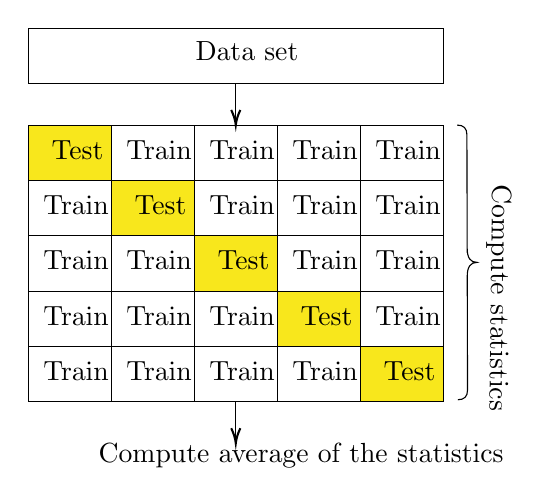
\begin{tikzpicture}[x=0.5pt,y=0.5pt,yscale=-1,xscale=1]
%uncomment if require: \path (0,487); %set diagram left start at 0, and has height of 487

%Shape: Rectangle [id:dp9628831478307318]
\draw   (90,20) -- (390,20) -- (390,60) -- (90,60) -- cycle ;
%Shape: Rectangle [id:dp40247556319098454]
\draw   (150,90) -- (210,90) -- (210,130) -- (150,130) -- cycle ;
%Straight Lines [id:da38673279994063514]
\draw    (240,60) -- (240,88) ;
\draw [shift={(240,90)}, rotate = 270] [color={rgb, 255:red, 0; green, 0; blue, 0 }  ][line width=0.75]    (10.93,-3.29) .. controls (6.95,-1.4) and (3.31,-0.3) .. (0,0) .. controls (3.31,0.3) and (6.95,1.4) .. (10.93,3.29)   ;
%Shape: Brace [id:dp44265578721237586]
\draw   (400.5,288.5) .. controls (405.17,288.49) and (407.49,286.15) .. (407.48,281.48) -- (407.28,199.23) .. controls (407.27,192.56) and (409.59,189.23) .. (414.26,189.22) .. controls (409.59,189.23) and (407.25,185.9) .. (407.23,179.23)(407.24,182.23) -- (407.03,96.98) .. controls (407.02,92.31) and (404.68,89.99) .. (400.01,90) ;
%Shape: Rectangle [id:dp6086176363319614]
\draw  [fill={rgb, 255:red, 248; green, 231; blue, 28 }  ,fill opacity=1 ] (90,90) -- (150,90) -- (150,130) -- (90,130) -- cycle ;
%Shape: Rectangle [id:dp6253670891530648]
\draw   (210,90) -- (270,90) -- (270,130) -- (210,130) -- cycle ;
%Shape: Rectangle [id:dp012463141021535118]
\draw   (270,90) -- (330,90) -- (330,130) -- (270,130) -- cycle ;
%Shape: Rectangle [id:dp03635717517805359]
\draw   (330,90) -- (390,90) -- (390,130) -- (330,130) -- cycle ;
%Shape: Rectangle [id:dp6139521323150046]
\draw   (90,130) -- (150,130) -- (150,170) -- (90,170) -- cycle ;
%Shape: Rectangle [id:dp2734748607023023]
\draw   (210,130) -- (270,130) -- (270,170) -- (210,170) -- cycle ;
%Shape: Rectangle [id:dp7416160208443594]
\draw   (270,130) -- (330,130) -- (330,170) -- (270,170) -- cycle ;
%Shape: Rectangle [id:dp04965387626199025]
\draw   (330,130) -- (390,130) -- (390,170) -- (330,170) -- cycle ;
%Shape: Rectangle [id:dp36390369464546923]
\draw   (90,170) -- (150,170) -- (150,210) -- (90,210) -- cycle ;
%Shape: Rectangle [id:dp0583337342908441]
\draw   (150,170) -- (210,170) -- (210,210) -- (150,210) -- cycle ;
%Shape: Rectangle [id:dp7518796244751725]
\draw   (270,170) -- (330,170) -- (330,210) -- (270,210) -- cycle ;
%Shape: Rectangle [id:dp8731512433065419]
\draw   (330,170) -- (390,170) -- (390,210) -- (330,210) -- cycle ;
%Shape: Rectangle [id:dp3374950674483356]
\draw   (90,210) -- (150,210) -- (150,250) -- (90,250) -- cycle ;
%Shape: Rectangle [id:dp2425800253901771]
\draw   (150,210) -- (210,210) -- (210,250) -- (150,250) -- cycle ;
%Shape: Rectangle [id:dp9764918971023423]
\draw   (210,210) -- (270,210) -- (270,250) -- (210,250) -- cycle ;
%Shape: Rectangle [id:dp3030426321919574]
\draw   (330,210) -- (390,210) -- (390,250) -- (330,250) -- cycle ;
%Shape: Rectangle [id:dp08910405765909535]
\draw   (90,250) -- (150,250) -- (150,290) -- (90,290) -- cycle ;
%Shape: Rectangle [id:dp3282550386553066]
\draw   (150,250) -- (210,250) -- (210,290) -- (150,290) -- cycle ;
%Shape: Rectangle [id:dp25498660930064765]
\draw   (210,250) -- (270,250) -- (270,290) -- (210,290) -- cycle ;
%Shape: Rectangle [id:dp08541585559965792]
\draw   (270,250) -- (330,250) -- (330,290) -- (270,290) -- cycle ;
%Shape: Rectangle [id:dp19772098788401882]
\draw  [fill={rgb, 255:red, 248; green, 231; blue, 28 }  ,fill opacity=1 ] (150,130) -- (210,130) -- (210,170) -- (150,170) -- cycle ;
%Shape: Rectangle [id:dp01839862708870832]
\draw  [fill={rgb, 255:red, 248; green, 231; blue, 28 }  ,fill opacity=1 ] (210,170) -- (270,170) -- (270,210) -- (210,210) -- cycle ;
%Shape: Rectangle [id:dp11813630833655397]
\draw  [fill={rgb, 255:red, 248; green, 231; blue, 28 }  ,fill opacity=1 ] (270,210) -- (330,210) -- (330,250) -- (270,250) -- cycle ;
%Shape: Rectangle [id:dp9995560009248317]
\draw  [fill={rgb, 255:red, 248; green, 231; blue, 28 }  ,fill opacity=1 ] (330,250) -- (390,250) -- (390,290) -- (330,290) -- cycle ;
%Straight Lines [id:da24602633489740156]
\draw    (240,290) -- (240,318) ;
\draw [shift={(240,320)}, rotate = 270] [color={rgb, 255:red, 0; green, 0; blue, 0 }  ][line width=0.75]    (10.93,-3.29) .. controls (6.95,-1.4) and (3.31,-0.3) .. (0,0) .. controls (3.31,0.3) and (6.95,1.4) .. (10.93,3.29)   ;

% Text Node
\draw (105,99) node [anchor=north west][inner sep=0.75pt]   [align=left] {Test};
% Text Node
\draw (159,99) node [anchor=north west][inner sep=0.75pt]   [align=left] {Train};
% Text Node
\draw (209,28) node [anchor=north west][inner sep=0.75pt]   [align=left] {Data set};
% Text Node
\draw (441.01,131.27) node [anchor=north west][inner sep=0.75pt]  [rotate=-90.74] [align=left] {Compute statistics};
% Text Node
\draw (139,318) node [anchor=north west][inner sep=0.75pt]   [align=left] {Compute average of the statistics};
% Text Node
\draw (219,99) node [anchor=north west][inner sep=0.75pt]   [align=left] {Train};
% Text Node
\draw (279,99) node [anchor=north west][inner sep=0.75pt]   [align=left] {Train};
% Text Node
\draw (339,99) node [anchor=north west][inner sep=0.75pt]   [align=left] {Train};
% Text Node
\draw (99,139) node [anchor=north west][inner sep=0.75pt]   [align=left] {Train};
% Text Node
\draw (219,139) node [anchor=north west][inner sep=0.75pt]   [align=left] {Train};
% Text Node
\draw (279,139) node [anchor=north west][inner sep=0.75pt]   [align=left] {Train};
% Text Node
\draw (339,139) node [anchor=north west][inner sep=0.75pt]   [align=left] {Train};
% Text Node
\draw (99,179) node [anchor=north west][inner sep=0.75pt]   [align=left] {Train};
% Text Node
\draw (159,179) node [anchor=north west][inner sep=0.75pt]   [align=left] {Train};
% Text Node
\draw (279,179) node [anchor=north west][inner sep=0.75pt]   [align=left] {Train};
% Text Node
\draw (339,179) node [anchor=north west][inner sep=0.75pt]   [align=left] {Train};
% Text Node
\draw (99,219) node [anchor=north west][inner sep=0.75pt]   [align=left] {Train};
% Text Node
\draw (159,219) node [anchor=north west][inner sep=0.75pt]   [align=left] {Train};
% Text Node
\draw (219,219) node [anchor=north west][inner sep=0.75pt]   [align=left] {Train};
% Text Node
\draw (339,219) node [anchor=north west][inner sep=0.75pt]   [align=left] {Train};
% Text Node
\draw (99,259) node [anchor=north west][inner sep=0.75pt]   [align=left] {Train};
% Text Node
\draw (159,259) node [anchor=north west][inner sep=0.75pt]   [align=left] {Train};
% Text Node
\draw (219,259) node [anchor=north west][inner sep=0.75pt]   [align=left] {Train};
% Text Node
\draw (279,259) node [anchor=north west][inner sep=0.75pt]   [align=left] {Train};
% Text Node
\draw (165,139) node [anchor=north west][inner sep=0.75pt]   [align=left] {Test};
% Text Node
\draw (225,179) node [anchor=north west][inner sep=0.75pt]   [align=left] {Test};
% Text Node
\draw (285,219) node [anchor=north west][inner sep=0.75pt]   [align=left] {Test};
% Text Node
\draw (345,259) node [anchor=north west][inner sep=0.75pt]   [align=left] {Test};


\end{tikzpicture}

                \caption{\label{fig: Cross Validation}Visual representation of $k$-fold cross-sampling for $k=5$}
            \end{figure}
            When doing cross-validation, typical choices of $k$ are $5$ and $10$ \cite{hastie}. Which one is better will depend on how the error scales with the size of the training set, as such, choosing a suitable $k$ requires some analysis.
            The cross-validation resampling provides a good estimate for the mean error of our estimates.
            \begin{itemize}
                \item Discuss this in more detail $\rightarrow\Delta Err$ wrt to number of data points
            \end{itemize}
        \subsubsection{Bootstrap}
            \noindent
            In the bootstrap resampling method, we sample our data set $S = \{s_1, \dots s_N\}$ $N$-number of times, in particular, we allow sampling the same $s_i$ multiple times. In this way, we generate new datasets in which some points are underweighted and others overweighted with respect to the original dataset $S$. So we effectively are generating small pertubations of the original dataset, which we may then use to compute new statistics.
            In particular, this technique enables us to investivate the variance of our model wrt small pertubations of the predictors. \textbf{This may be worded more elegantly}
            \begin{itemize}
                \item touch on rates of convergence
            \end{itemize}

    \subsection{The Bias-Variance Tradeoff}

\section{Results}

\section{Discussion}

\section{Conclusion}

\onecolumngrid
\bibliography{bibfile}
\newpage
\twocolumngrid
\appendix


\end{document}
